% This is samplepaper.tex, a sample chapter demonstrating the
% LLNCS macro package for Springer Computer Science proceedings;
% Version 2.20 of 2017/10/04
%
\documentclass[runningheads,table]{llncs}
%
\usepackage{graphicx}

% For algorithmic attachments and graphics
\usepackage{amsmath}
\usepackage{amssymb}
\usepackage{algorithm}
\usepackage{algorithmicx}
\usepackage[noend]{algpseudocode}
\usepackage{subcaption}
\captionsetup{compatibility=false}

\usepackage{tikz}
\usepackage{dsfont}
\usepackage{multicol, multirow}
\usepackage{textcomp}
%\usepackage{booktabs}
\usetikzlibrary{fit,calc,automata,positioning}

\usepackage{kbordermatrix}
\usepackage{extarrows}
\usepackage{balance}
\usepackage{colortbl}
\usepackage{mathtools}
\usepackage{verbatim}
\definecolor{lightgray}{gray}{0.9}



% Used for displaying a sample figure. If possible, figure files should
% be included in EPS format.
%
% If you use the hyperref package, please uncomment the following line
% to display URLs in blue roman font according to Springer's eBook style:
% \renewcommand\UrlFont{\color{blue}\rmfamily}

\newtheorem{mytheorem}{Theorem}
\newtheorem{myproposition}{Proposition}

\newcommand{\ltz}{$< 1$}

\algtext*{EndWhile}% Remove "end while" text
\algtext*{EndIf}% Remove "end if" text
\algtext*{EndFor}% Remove "end for" text
\algtext*{EndFunction}% Remove "end function" text

\begin{document}
%
\title{Multiple Context-Free Path Querying by Matrix Multiplication\thanks{The research was supported by the Russian Science Foundation, grant \textnumero 18-11-00100}}
%
%\titlerunning{Abbreviated paper title}
% If the paper title is too long for the running head, you can set
% an abbreviated paper title here
%
\author{Ilya Epelbaum\inst{1} \and
Rustam Azimov\inst{1,2} \and
Semyon~Grigorev\inst{1,2}\orcidID{0000-0002-7966-0698}}
%
\authorrunning{I. Epelbaum et al.}
% First names are abbreviated in the running head.
% If there are more than two authors, 'et al.' is used.
%
\institute{St.Petersburg State University, 7/9 Universitetskaya nab., St. Petersburg, Russia, 199034 \\
\email{iliyepelbaun@gmail.com, rustam.azimov19021995@gmail.com, s.v.grigoriev@spbu.ru} \and
JetBrains Research, Primorskiy prospekt 68-70, Building 1, St. Petersburg, Russia, 197374}
%
\maketitle              % typeset the header of the contribution
%
\begin{abstract}
Many graph analysis problems can be formulated as formal language-constrained path querying problems where the formal languages are used as constraints for
navigational path queries. Recently, the context-free language (CFL) reachability formulation has become very popular and can be used in many areas, for example, querying graph databases, RDF analysis, static code analysis, biological data analysis, graph segmentation. However, the generative capacity of context-free grammars (CFGs) is too weak to generate some complex queries, for example, from natural languages, and the various extensions of CFGs have been proposed. Multiple context-free grammar (MCFG) is one of such extensions of CFGs. Despite the fact that, to the best of our knowledge, there is no algorithm for MCFL-reachability, this problem is known to be decidable. The creation of the MCFL-reachability algorithms allows one to use more complex graph queries that may find application in various areas, for example, in static code analysis. In this paper, we provide the first MCFL-reachability algorithm that also is based on Boolean matrix multiplication. Thus, the proposed algorithm can be implemented by using high-performance libraries and modern parallel hardware.


\keywords{Multiple context-free path querying \and Graph database \and RDF \and Multiple context-free grammars \and Boolean matrix multiplication \and GraphBLAS API.}
\end{abstract}
%
%
%

\section{Introduction}

Scalable high-performance graph analysis is an actual challenge.
There is a big number of ways to attack this challenge~\cite{Coimbra2021} and the first promising idea is to utilize general-purpose graphic processing units (GPGPU).
Such existing solutions, as CuSha~\cite{10.1145/2600212.2600227} and Gunrock~\cite{7967137} show that utilization of GPUs can improve the performance of graph analysis, moreover it is shown that solutions may be scaled to multi-GPU systems.
But low flexibility and high complexity of API are problems of these solutions.

The second promising thing which provides a user-friendly API for high-performance graph analysis algorithms creation is a GraphBLAS API~\cite{7761646} which provides linear algebra based building blocks to create graph analysis algorithms.
The idea of GraphBLAS is based on a well-known fact that linear algebra operations can be efficiently implemented on parallel hardware.
Along with that, a graph can be natively represented using matrices: adjacency matrix, incidence matrix, etc.
While reference CPU-based implementation of GraphBLAS, SuiteSparse:GraphBLAS~\cite{10.1145/3322125}, demonstrates good performance in real-world tasks, GPU-based implementation is challenging.

One of the challenges in this way is that real data are often sparse, thus underlying matrices and vectors are also sparse, and, as a result, classical dense data structures and respective algorithms are inefficient. 
So, it is necessary to use advanced data structures and procedures to implement sparse linear algebra, but the efficient implementation of them on GPU is hard due to the irregularity of workload and data access patterns.
Though such well-known libraries as cuSPARSE show that sparse linear algebra operations can be efficiently implemented for GPGPU, it is not so trivial to implement GraphBLAS on GPGPU. 
First of all, it requires \textit{generic} sparse linear algebra, thus it is impossible just to reuse existing libraries which are almost all specified for operations over floats.
The second problem is specific optimizations, such as masking fusion, which can not be natively implemented on top of existing kernels.
Nevertheless, there is a number of implementations of GraphBLAS on GPGPU, such as GraphBLAST~\cite{yang2019graphblast}, GBTL~\cite{7529957}, which show that GPGPUs utilization can improve the performance of GraphBLAS-based graph analysis solutions.
But these solutions are not portable because they are based on Nvidia Cuda stack.
Moreover, the scalability problem is not solved: all these solutions support only single-GPU, not multi-GPU computations.

To provide portable GPU implementation of GraphBLAS API we developed a \textit{SPLA} library\footnote{Source code available at: \url{https://github.com/JetBrains-Research/spla}}.
This library utilizes OpenCL for GPGPU computing to be portable across devices of different vendors.
Moreover, it is initially designed to utilize multiple GPGPUs to be scalable.
To sum up, the contribution of this work is the following.
\begin{itemize}
    \item Design of portable GPU GraphBLAS implementation proposed. The design involves the utilization of multiple GPUS. Additionally, the proposed design is aimed to simplify library tuning and wrappers for different high-level platforms and languages creation. 
    \item Subset of GraphBLAS API, including such operations as masking, matrix-matrix multiplication, matrix-matrix e-wise addition, is implemented. The current implementation is limited by COO and CSR matrix representation format and uses basic algorithms for some operations, but work in progress and more data formats will be supported and advanced algorithms will be implemented in the future.
    \item Preliminary evaluation on such algorithms as breadth-first search (BFS) and triangles counting (TC), and real-world graphs shows portability across different vendors and promising performance: for some problems Spla is comparable with GraphBLAST. Surprisingly, for some problems, the proposed solution on embedded Intel graphic card shows better performance than SuiteSparse:GraphBLAS on the respective CPU. At the same time, the evaluation shows that further optimization is required.
\end{itemize} 
\section{Preliminaries}

In this section we introduce common definitions in graph theory and formal language theory which will be used in this paper. 
Also, we provide brief description of Azimov's algorithm which is used as a base of our solution.

\subsection{Graphs}

In this work we use edge-labelled digraph as a data model and define it as follows.
\begin{definition} \emph{Labeled directed graph} is a triple $D = (V,E,\sigma)$, where
\begin{itemize}
    \item $V$ is a set of vertices
    \item $E$ is a set of edges
    \item $\sigma \subseteq \Sigma$ is a set of labels, and a set of edges $E\subseteq V\times \sigma \times V$
\end{itemize}
\end{definition}

An example of the graph is presented in figure~\ref{fig:example_input_graph}.

\begin{figure}[h]
    \centering        
    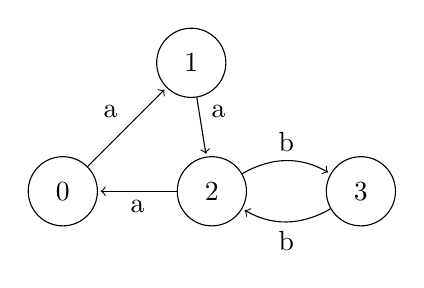
\begin{tikzpicture}[shorten >=1pt,auto]
       \node[state] (q_0)                      {$0$};
       \node[state] (q_1) [above right=of q_0] {$1$};
       \node[state] (q_2) [right=of q_0]       {$2$};
       \node[state] (q_3) [right=of q_2]       {$3$};
        \path[->]
        (q_0) edge  node {a} (q_1)
        (q_1) edge  node {a} (q_2)
        (q_2) edge  node {a} (q_0)
        (q_2) edge[bend left, above]  node {b} (q_3)
        (q_3) edge[bend left, below]  node {b} (q_2);
    \end{tikzpicture}
    \caption{The example of input graph $\mathcal{G}$}
    \label{fig:example_input_graph}
\end{figure}

We use adjacency matrix decomposed to a set of a boolean matrix as a representation of the graph.
\begin{definition}
An adjacency matrix $M$ of the graph $\mathcal{G}=$ is a square $|V|\times|V|$ matrix, such that $M[i,j] = \{l \mid e = (i,l,j) \in E\}$.
\end{definition}

Adjacency matrix $M$ of the graph $\mathcal{G}$ is

$$
    M =
    \begin{pmatrix}
    . & \{a\} & . & .     \\
    . & . & \{a\} & .     \\
    \{a\} & . & . & \{b\} \\
    . & . & \{b\} & .
    \end{pmatrix}.
$$

\begin{definition}

Boolean decomposition of adjacency matrix $M$ of graph $\mathcal{G}=$ is set of Boolean matrix $$\mathcal{M} = \{M^l \mid l \in L, M^l[i,j]=1 \iff l \in M[i,j]\}.$$

\end{definition}

Matrix $M$ can be represented as a set of two Boolean matrices $M^a$ and $M^b$ where
\begin{align}
M^{a} =
\begin{pmatrix}
    . & 1 & . & .   \\
    . & . & 1 & .   \\
    1 & . & . & .   \\
    . & . & . & .  
\end{pmatrix}, 
M^{b} =
\begin{pmatrix}      
    . & . & . & .   \\
    . & . & . & .   \\
    . & . & . & 1   \\
    . & . & 1 & . 
\end{pmatrix} \label{eq:boolean_decomposition_of_graph}
\end{align}
\subsection{Languages}

\begin{definition}\emph{Context-free grammar} is a 4-tuple $G=(N, \Sigma, R, S)$, where 
\begin{itemize}
    \item $N$ is a set of nonterminals
    \item $\Sigma$ is a set of terminals
    \item $R$ is a finite set of productions of the followings form: $A \to \alpha, ~A \in N,~ \alpha \in (N \cup \Sigma)^*$
    \item $S$ - a starting nonterminal
\end{itemize}
\end{definition}

\begin{definition} \emph{Context-free language} is a language generated by a context-free grammar:
\begin{align*}
     L(G) = \{w \in \Sigma^* \mid S \Rightarrow^* w \} 
\end{align*}
Where $S \Rightarrow^* w$  denotes that a string $w$ can be generated from a starting non-terminal $S$ using some sequence of production rules from $P$.
\end{definition}

\begin{definition} Context-free grammar $G = (N, \Sigma, R, S)$ is said to be in \emph{Chomsky normal form} if all productions in $R$ are of the form:
    \begin{itemize}
        \item $A \rightarrow BC,~A,~B,~C \in N$
        \item  $A \rightarrow a,~A \in N,~a \in \Sigma$
        \item $S \rightarrow \varepsilon,~\varepsilon$ is an empty string
    \end{itemize}
\end{definition}
Note that every context-free grammar can be transformed into an equivalent one in Chomsky Normal Form. 
\begin{definition} Context-free grammar $G = (N, \Sigma, P, S)$ is said to be in \emph{Weak Chomsky normal form} if all productions in $P$ are of the form:
    \begin{itemize}
        \item $A \rightarrow BC,~A,~B,~C \in N$
        \item  $A \rightarrow a,~A \in N,~a \in \Sigma$
        \item $A \rightarrow \varepsilon,~A \in N$
    \end{itemize}
\end{definition}
In other words, weak Chomsky normal form differs from Chomsky normal Form in the followings:
\begin{itemize}
    \item $\varepsilon$ can be derived from any non-terminal
    \item $S$ can be at a right part of productions
\end{itemize}
    
    
For example, let's consider the following context-free grammar, which generates the language $L(G) = \{A^nB^n, n \in \mathbb{N}\}$:
$G=(N, \Sigma, P, S), ~N=\{S\},~\Sigma=\{A,B\}$ and productions: 
\begin{align*}
S \rightarrow AB \\
S \rightarrow ASB\\
S \rightarrow \varepsilon
\end{align*}
After transformation to Chomsky Normal Form the resulting grammar:
\begin{align*}
S \rightarrow AB \\
S \rightarrow AC \\
C \rightarrow SB \\
S \rightarrow \varepsilon
\end{align*}

This productions itself are the grammar that has the same result as original grammar.

We use a context-free grammar in the weak Chomsky Normal Form without a starting non-terminal, which will be specified in the path queries for the graph. It should be noted that we omit the rules of the form $A \rightarrow \varepsilon$ for the reason that they correspond to trivial paths, which are more convenient to consider separately.

\begin{definition}\emph{Context-free relation} is a relation $R_A \subseteq V \times V$ for graph $G = (V, E)$, context-free grammar $G = (N,~\Sigma,~P)$ and fixed non-terminal $A$:
\begin{align*}
     R_A = \{(n, m) \mid \exists n \pi m~(l(\pi) \in L(G_A))\}
\end{align*}
\end{definition}

 Now, the definition for \emph{multiple-source (single-source) context-free path querying problem} can be formulated in the introduced notation as follows. For the given graph $G = (V, E)$, context-free grammar $G=(N, \Sigma, P)$ and set of source vertices $Src$ we need to find all context-free relations $R_A$ for any $A \in Src$. 
 
\subsection{Matrix-Based Algorithm}
Let $D = (V, E)$ be the input graph and $G = (N, \Sigma, P)$ be the input grammar. For the context-free path query evaluation, we need to provide context-free relations \mbox{$R_A \subseteq V \times V$} for every \mbox{$A \in N$}.
The matrix-based algorithm for CFPQ can be expressed in terms of operations over Boolean matrices (see listing~\ref{alg:algo0}) which is an advantage for implementation.
{\footnotesize
\begin{algorithm}
\begin{algorithmic}[1]
\caption{Context-free path querying algorithm}
\label{alg:algo0}
\Function{evalCFPQ}{$D=(V,E), G=(N,\Sigma,P)$}
    \State{$n \gets$ |V|}
    \State{$T \gets \{T^{A_i} \mid A_i \in N, T^{A_i}$ is a matrix $n \times n$, $T^{A_i}_{k,l} \gets$ \texttt{false}\} }
    \ForAll{$(i,x,j) \in E$, $A_k \mid A_k \to x \in P$}
        %\Comment{Matrices initialization}
        %\For{$A_k \mid A_k \to x \in P$}
          {$T^{A_k}_{i,j} \gets \texttt{true}$}
        %\EndFor
    \EndFor
    \ForAll{$A_k \mid A_k \to \varepsilon \in P$}
        \ForAll{$i \in \{0,\ldots ,n-1\}$}
            {$T^{A_k}_{i,i} \gets \texttt{true}$}
        \EndFor
    \EndFor

    \While{any matrix in $T$ is changing}
        %\Comment{Transitive c	losure calculation}
        \For{$A_i \to A_j A_k \in P$}
          { $T^{A_i} \gets T^{A_i} + (T^{A_j} \times T^{A_k})$ } 
        \EndFor
    \EndWhile
\State \Return $T$
\EndFunction
\end{algorithmic}
\end{algorithm}
}

This CFPQ algorithm allows efficiently apply GPGPU techniques, but it solves all-pairs problem and takes unreasonable amount of memory in scenarios in which we want to find paths from a relatively small set of vertices, since it calculates a lot of redundant information.  
\section{Механизм диагностики ошибок}
Предлагаемый механизм диагностики ошибок состоит из двух частей:
\begin{itemize}
    \item алгоритм синтаксического анализа регулярной аппроксимации динамически формируемых выражений (далее основной анализ) модифицируется, позволяя для каждой GSS вершины строить все корректные для нее префиксы внутреннего графа;
    \item после основного анализа с помощью построенных префиксов обнаруживаются ошибочные ребра внутреннего графа.
\end{itemize}
Далее в этой главе будут рассмотрены: компактное представление префиксов внутреннего графа, алгоритм построения корректных префиксов внутреннего графа для GSS-вершин и алгоритм диагностики ошибок, проводящий анализ построенных префиксов.

\subsection{Компактное представление префиксов внутреннего графа}
Так как внутренний граф может иметь циклы, то множество различных префиксов внутреннего графа может быть бесконечным. В качестве компактного представления всех корректных префиксов внутреннего графа для вершины GSS используется ориентированный граф с выделенным множеством начальных вершин (далее \emph{граф префиксов}). Из-за особенностей операций, используемых при построении графов префиксов, начальные вершины представляют не начало, а конец хранимых префиксов внутреннего графа в рассматриваемом графе префиксов. Каждая вершина в графе префиксов ассоциируется с ребром GSS или является специальной вершиной $EOP$ (End Of Prefix). Ребра GSS, в свою очередь, будем делить на три вида:
\begin{itemize}
    \item  \emph{терминальное} ребро --- ребро, порожденное операцией сдвига по какому-то терминалу $t$;
    \item \emph{нетерминальное} --- ребро, порожденное операцией свертки длины $l$, где $l > 0$;
    \item \emph{обнуляемое} --- ребро, порожденное операцией свертки длины $l$, где $l = 0$.
\end{itemize}
Будем говорить, что начальная вершина $V$ графа префиксов $GP_{1}$ \emph{соединена} с графом префиксов $GP_{2}$, если для любой начальной вершины $U$ графа префиксов $GP_{2}$, существует ребро из вершины $V$ в вершину $U$. Каждая, кроме $EOP$, начальная вершина графа префиксов соединена с одним графом префиксов. Вершина $EOP$ не имеет исходящих дуг.

С каждым нетерминальным ребром ассоциируется множество путей в GSS, по которым произведена операция свертки для данного нетерминального ребра. Будем говорить что данное нетерминальное ребро \emph{порождает} каждый путь из рассмотренного множества путей GSS.
% * <Екатерина Вербицкая> 14:16:56 13 May 2016 UTC+0300:
% > множество путей в GSS, по которым произведена операция свертки
% 
% Я не уверена, что так говорить корректно.

Рассмотрим путь $(V_{1},..,V_{n})$ в графе префиксов $GP$ как последовательность вершин графов префиксов. Удалим вершину $EOP$, если она присутствует, а также заменим все вершины в данном пути на ребра GSS, с которыми они ассоциируются. Получим последовательность $(e_{1},..,e_{n})$ ребер GSS. \emph{Раскрытием} данной последовательности будем называть последовательность, получающуюся в результате применения следующих действий:
\begin{itemize}
    \item все нетерминальные ребра GSS $e$, заменяются на последовательность ребер, соответствующую одному из порожденных ребром $e$ пути;
    \item все обнуляемые ребра GSS удаляются из последовательности.
\end{itemize}
Если после конечного числа раскрытий в последовательности останутся только терминальные ребра GSS, то будем говорить, что изначальный путь в графе префиксов \emph{сводится} к строке, получающейся инвертированием этой последовательности терминальных ребер и их замены на терминалы, с которыми они ассоциированы. Если полученная строка получается заменой ребер в пути префикса внутреннего графа $P$, на терминалы, которыми нагружены эти ребра, то путь в графе префиксов \emph{сводится} к префиксу внутреннего графа $P$. Будем говорить, что граф префиксов $GP$ \emph{порождает} префикс внутреннего графа $P$, если $\exists (V_{1},..,V_{n},EOP)$ --- путь в графе префиксов $GP$, где $V_{1}$ --- одна из начальных вершин графа префиксов $GP$, который сводится к префиксу внутреннего графа $P$. В графе префиксов также могут быть циклы, что позволяет сводиться к бесконечному множеству префиксов внутреннего графа.
% * <Екатерина Вербицкая> 14:24:18 13 May 2016 UTC+0300:
% Сюда бы тоже картинку.

\subsection{Алгоритм построения префиксов}
Данный алгоритм является модификацией алгоритма ослабленного синтаксического анализа регулярной аппроксимации динамически формируемого выражения. Добавляется ассоциация вершин GSS с коллекцией $prefixes$ --- граф префиксов, порождающий все корректные префиксы внутреннего графа для данной GSS вершины. После создания начальной GSS-вершины в ее графе префиксов создается начальная вершина $EOP$. Добавляется ассоциация нетерминальных ребер GSS с коллекцией $paths$ --- множество путей в GSS, порождаемых рассматриваемым нетерминальным ребром. Функция $addEdge$ модифицируется, добавляется дополнительный параметр $pathsToAdd$ --- множество путей в GSS, которое необходимо добавить к множеству путей в GSS, порождаемых ребром $edge$ из вершины $v_{t}$ в вершину $v_{h}$. Также создается начальная вершина графа префиксов $v_{t}.prefixes$, ассоциированная с ребром $edge$ и соединенная с графом префиксов $v_{h}.prefixes$. Функция $addVertex$ не изменилась.

\begin{algorithm}[H]
\begin{algorithmic}[1]
\caption{Модификация построения GSS}
\label{addEdge_mod}
\Function{addEdge}{$v_{h}, innerGraphV, state_{t}, isZeroReduction, pathsToAdd$}

  \State{$(v_{t}, isNew) \gets$ \Call{addVertex}{$innerGraphV, state_{t}$}}
  \If{GSS does not contain edge from $v_{t}$ to $v_{h}$}
% * <Екатерина Вербицкая> 14:26:52 13 May 2016 UTC+0300:
% Может тут тоже можно половину кода выкинуть, оставив только важное.
% ^ <Рустам Азимов> 14:27:51 13 May 2016 UTC+0300:
% Не представляю пока. Как это?
    \State{$edge \gets$ create new edge from $v_{t}$ to $v_{h}$}
    \State{$\mathcal{Q}.Enqueue(innerGraphV)$}
    \If{not $isNew$ and $v_{t}.passingReductions.Count>0$}
      \State{add $(v_{t}, edge)$ in $innerGraphV.passingReductionsToHandle$}
    \EndIf
    \If{not $isZeroReduction$}
      \ForAll{$e$ in outgoing edges of $innerGraphV$}
        \State{calculate the set of reductions by $v$ and the token on $e$}
        \State{     and add them in $innerGraphV.reductions$}
      \EndFor
    \EndIf
    \State{$V \gets$ vertex of the prefix graph,}
    \State{     associated with $edge$ and connected to $v_{h}.prefixes$}
    \State{add $V$ to initial vertexes of $v_{t}.prefixes$}
  \EndIf
  \If{pathsToAdd is not empty}
    \State{$edge \gets$ edge from $v_{t}$ to $v_{h}$}
    \State{add all paths in $pathsToAdd$ to $edge.paths$}
  \EndIf
\EndFunction
\end{algorithmic}
\end{algorithm}

Параметр $pathsToAdd$ при вызове функции $addEdge$ для терминальных или обнуляемых ребер GSS является пустым множеством.

\begin{algorithm}[H]
\begin{algorithmic}[1]
\caption{Модификация операции сдвига}
\label{push_mod}
\Function{push}{$innerGraphV$}
  \State{$\mathcal{U} \gets$ copy $innerGraphV.unprocessed$}
  \State{clear $innerGraphV.unprocessed$}
  \ForAll{$v_{h}$ in $\mathcal{U}$}  
    \ForAll{$e$ in outgoing edges of $innerGraphV$}
      \State{$push \gets$ calculate next state by $v_{h}.state$ and the token on $e$}
      \State{$pathsToAdd \gets$ empty set}
% * <Екатерина Вербицкая> 14:32:07 13 May 2016 UTC+0300:
% Обычно в таких листингах новый код выделяется болдом или еще как-то в том же духе. Чтобы повысить читабельность и чтобы сразу было понятно, что конкретно изменилось.
      \State{\Call{addEdge}{$v_{h}, e.Head, push, false, pathsToAdd$}}
      \State{add $v_{h}$ in $innerGraphV.processed$}
    \EndFor
  \EndFor
\EndFunction
\end{algorithmic}
\end{algorithm}

\begin{algorithm}[H]
\begin{algorithmic}[1]
\caption{Модификация операции свертки}
\label{reduce_mod}
\Function{makeReductions}{$innerGraphV$}
  \While{$innerGraphV.reductions$ is not empty}
    \State{$(startV, N, l) \gets innerGraphV.reductions.Dequeue()$}
    \State{find the set of vertices $\mathcal{X}$ reachable from $startV$}
    \State{    along the path of length ($l-1$), or $0$ if $l=0$;}
    \State{add $(startV, N, l-i)$ in $v.passingReductions$,}
    \State{    where $v$ is an $i$-th vertex of the path}
    \ForAll{$v_{h}$ in $\mathcal{X}$}
      \State{$state_{t} \gets$ calculate new state by $v_{h}.state$ and nonterminal $N$}
      \If{$l > 0$}
        \State{$pathsToAdd \gets$ all paths, by which $v_{h}$ is reachable}
        \State{     from $startV$}
      \Else
        \State{$pathsToAdd \gets$ empty set}
      \EndIf
      \State{\Call{addEdge}{$v_{h}, startV, state_{t}, (l=0), pathsToAdd$}}
    \EndFor
  \EndWhile
\EndFunction

\Function{applyPassingReductions}{$innerGraphV$}
  \ForAll{$(v, edge)$ in $innerGraphV.passingReductionsToHandle$}
    \ForAll{$(startV, N, l) \gets v.passingReductions.Dequeue()$}
      \State{find the set of vertices $\mathcal{X}$,}
      \State{    reachable from $edge$ along the path of length ($l-1$)}
      \ForAll{$v_{h}$ in $\mathcal{X}$}
        \State{$state_{t} \gets$ calculate new state by $v_{h}.state$ and nonterminal $N$}
        \State{$pathsToAdd \gets$ all paths, by which $v_{h}$ is reachable}
        \State{     from $startV$}
        \State{\Call{addEdge}{$v_{h}, startV, state_{t}, false, pathsToAdd$}}
      \EndFor
    \EndFor
  \EndFor
\EndFunction
\end{algorithmic}
\end{algorithm}

После описанных модификаций алгоритм синтаксического анализа регулярной аппроксимации динамически формируемого выражения для каждой вершины GSS дополнительно конструирует все корректные для нее префиксы внутреннего графа.

\subsection{Алгоритм диагностики ошибок}
Данный алгоритм получает на вход внутренний граф с построенными в ходе основного синтаксического анализа структурами (в том числе и префиксами внутреннего графа GSS вершин), а также сгенерированные RNGLR-таблицы. Алгоритм делает обход внутреннего графа и для каждого исходящего из вершины внутреннего графа ребра анализирует множества графов префиксов соседних вершин. 

Для обхода внутреннего графа используется глобальная очередь $Q$. Все ребра внутреннего графа, ведущие не в конечную вершину, обрабатываются в функции $processVertex$. Для ребер, ведущих в конечную вершину внутреннего графа, используется глобальная очередь $F$, с последующей обработкой в функции $processEOF$.

В результате работы алгоритма все ребра из множества $errors$ являются ошибочными, а ребра из множества $probErrors$ --- возможно ошибочными. То есть множество всех ошибочных ребер принадлежит объединению двух данных множеств. Кроме того, с элементами этих множеств ассоциируются множества графов префиксов (элемент $e$ множества $errors$ или множества $probErrors$ ассоциируется со множеством $errors[e]$ или $probErrors[e]$ соответственно), которые порождают корректные префиксы, заканчивающиеся в вершине, из которой исходит рассматриваемое ребро. Данные множества могут быть использованы при создании сообщения пользователю о возможных ошибках динамически формируемого выражения. Все префиксы, порождаемые графами префиксов из множества $errors[e]$, становятся некорректными при добавлении в конец ребра $e$. Все префиксы, порождаемые графами префиксов из множества $probErrors[e]$, возможно становятся некорректными при добавлении в конец ребра $e$. Но множество всех корректных префиксов внутреннего графа, заканчивающихся в вершине, из которой исходит ребро $e$, и становящихся некорректными при добавлении ребра $e$ в конец, порождается хотя бы одним графом префиксов из объединения множеств $errors[e]$ и $probErrors[e]$, где множество $errors[e]$ пусто, если $e \notin errors$, и множество $probErrors[e]$ пусто, если $e \notin probErrors$.
% * <Екатерина Вербицкая> 14:37:32 13 May 2016 UTC+0300:
% Что такое возможно ошибочные ребра? Почему множество всех ошибок -- это множество ошибок плюс возможно ошибочные?

\begin{algorithm}[H]
\begin{algorithmic}[1]
\caption{Алгоритм диагностики ошибок}
\label{error_handling}
\Function{findErrors}{$inputGraph, parserSource$}
    \State{$\mathcal{Q}.Enqueue(inputGraph.startVertex)$}
    \While{$Q$ is not empty}
        \State{$v \gets \mathcal{Q}.Dequeue()$}
        \State{\Call{processVertex}{$v$}}
    \EndWhile
    \While{$F$ is not empty}
        \State{$e \gets \mathcal{F}.Dequeue()$}
        \State{\Call{processEOF}{$e$}}
    \EndWhile
\EndFunction
\end{algorithmic}
\end{algorithm}

\begin{algorithm}[H]
\begin{algorithmic}[1]
\caption{Анализ неконечных ребер внутреннего графа}
\label{error_edges}
\Function{processVertex}{$innerGraphV$}
    \ForAll{$e$ in outgoing edges of $innerGraphV$}
        \If{token on $e$ is EOF}
            \State{$\mathcal{F}.Enqueue(e)$}
        \Else
            \If{$e.Head$ was not processed}
                \State{$\mathcal{Q}.Enqueue(e.Head)$}
            \EndIf
            \State{$headPrefixes \gets$ all prefixes graphs}
            \State{    from all GSS vertexes of $e.Head$;}
            \State{$pushedPrefixes \gets$ all prefixes graphs, to which connected}
            \State{    some initial vertex of prefixes graph in $headPrefixes$,}
            \State{     associated with terminal edge;}
            \State{$withCycle \gets$ all cyclical prefixes graphs in $pushedPrefixes$}
            \State{$withoutCycle \gets$ all non-cyclical graphs in $pushedPrefixes$}
            \State{$notPushedPrefixes \gets$ all prefixes graphs}
            \State{     from all GSS vertexes of $innerGraphV$,}
            \State{     without prefixes graphs from $pushedPrefixes$;}
            \ForAll{$p$ in $notPushedPrefixes$}
                \If{prefixes graph $p$ has a cycle}
                    \State{add $e$ to $probErrors$}
                    \State{add $p$ to $probErrors[e]$}
                \Else
                    \ForAll{$prefixPath$ in paths of prefixes graph $p$}
                        \State{$pathG \gets$ prefixes graph generated by $prefixPath$}
                        \If{$withoutCycle$ does not have any prefixes graph with
                            \State{    equivalent to $prefixPath$ path} }
                            \If{$withCycle$ is not empty}
                                \State{add $e$ to $probErrors$}
                                \State{add $pathG$ to $probErrors[e]$}
                            \Else
                                \State{add $e$ to $errors$}
                                \State{add $pathG$ to $errors[e]$}
                            \EndIf
                        \EndIf
                    \EndFor
                \EndIf
            \EndFor
        \EndIf
    \EndFor
\EndFunction
\end{algorithmic}
\end{algorithm}

\begin{algorithm}[H]
\begin{algorithmic}[1]
\caption{Анализ конечных ребер внутреннего графа}
\label{error_EOFedges}
\Function{processEOF}{$edge$}
    \State{$acceptedPrefixes \gets$ all prefixes graphs}
    \State{    from all GSS vertexes of $edge.Tail$ with accepted state;}
    \State{$withCycle \gets$ all cyclical prefixes graphs in $acceptedPrefixes$}
    \State{$withoutCycle \gets$ all non-cyclical graphs in $acceptedPrefixes$}
    \State{$notAcceptedPrefixes \gets$ all prefixes graphs}
    \State{    from all GSS vertexes of $edge.Tail$ with not accepted state;}
    \ForAll{$p$ in $notAcceptedPrefixes$}
        \If{prefixes graph $p$ has a cycle}
            \State{add $edge$ to $probErrors$} 
% * <Екатерина Вербицкая> 14:42:34 13 May 2016 UTC+0300:
% Вообще наличие цикла не говорит о том, что у нас обязательно в нем ошибка, поэтому нужна хоть какая-то мотивация в пользу такого подхода.
            \State{add $p$ to $probErrors[edge]$}
        \Else
            \ForAll{$prefixPath$ in paths of prefixes graph $p$}
                \State{$pathG \gets$ prefixes graph generated by $prefixPath$}
                \If{$withoutCycle$ does not have any prefixes graph 
                    \State{     with equivalent to $prefixPath$ path} }
                    \If{$withCycle$ is not empty}
                        \State{add $edge$ to $probErrors$}
                        \State{add $pathG$ to $probErrors[edge]$}
                    \Else
                        \State{add $edge$ to $errors$}
                        \State{add $pathG$ to $errors[edge]$}
                    \EndIf
                \EndIf
            \EndFor
        \EndIf
    \EndFor
\EndFunction
\end{algorithmic}
\end{algorithm}


\section{Evaluation}

This section describes the methodology and answers the following research questions.

\begin{enumerate}
    \item Does fusion via distillation give any benefits at the software and hardware levels?
    \item What are the properties of the generated hardware?
    \item Does the generated hardware outperform software implementations?
\end{enumerate}

\subsection{Methodology}

Our focus is on creating a basis for future research and experiments, thus we make our experiments as much reproducible as possible\footnote{\url{https://github.com/sedwards-lab/fhw/tree/sparse-linear-algebra-distillation/examples/QTreeBenchmarks/diploma/verilog-bool-no-nnz-inlined} (online; accessed:
2022-06-07) Here one could find all the results. For each benchmark all statistics are specified: matrix names, their sizes, collected metrics for both hardware and software benchmarks.}. We benchmarked the following list of chained functions. The choice is prompted by the current state of the distiller: at the moment, it does not successfully distill matrix multiplication. However, the functions are still practical enough, for example, chained addition could be seen in Luby's maximal independent set algorithm and clearly describe the applicability of the proposed approach.

\begin{itemize}
    \item \mintinline{Haskell}{mAdd (==False) (||) (mAdd (==False) (||) m1 m2) m3}
    \item \mintinline{Haskell}{mask (mAdd (== False) (||) m2 m3) (m1)}
    \item \mintinline{Haskell}{map (==Zero) (to_nat) (mAdd (==False) (||) m1 m2}
    \item \mintinline{Haskell}{map (==Zero) (to_nat) (kron (==False) (&&) m1 m2}
\end{itemize}

Above, \mintinline{Haskell}{Zero} and \texttt{to\_nat} are corresponding definitions for Peano arithmetics, since the \texttt{.pot} language does not have any primitives. For the same reason, we operated with boolean matrices. Such functions could be abstracted with free variables and then instantiated in the emitted Haskell code. However, to get maximum from distillation, we provided all the information about the functions. 

For these functions, we compared the execution time of distilled and not distilled hardware generated circuits, execution time of original and distilled Haskell code and reference \textit{Suite Sparse}\footnote{\url{https://github.com/DrTimothyAldenDavis/GraphBLAS} (online; accessed:
2022-06-07), Suite Sparse library sources.}\textsuperscript{,}\footnote{The library also uses different variations of coordinate formats (opaque to the user) and not a quadtree representation.} variants of these functions in C\texttt{++}. Note that SuiteSparse does not support recursive data types, thus only the first two function chains were implemented in SuiteSparse (since Peano number is essentially a linked list). We did not replace Peano numbers with integers, so our experiments could be interpreted easier. For hardware experiments we collected execution time and the number of memory writes and reads, to access how well fusion is performed. For software experiments we only measured the execution time. Also note that we measured only the time, required to execute the lines above, not including any IO, required to get and evaluate function arguments. But in hardware benchmarks we measured the time required to pass arguments into the circuit's memory, because such IO is inevitable. It is tricky to make such measures in Haskell due to laziness, thus the programs were compiled with \texttt{--fno-full-laziness} to turn off memoization. Also all the arguments were forced to normal form via \texttt{force} and \texttt{evaluate}. Haskell programs were compiled\footnote{GHC 8.10.4.} with \texttt{-O2 --fno-full-laziness} and Suite Sparse was compiled with default flags and linked as a shared library to C\texttt{++} code.

We took matrices from SuiteSparse matrix collection with sizes ranging from \texttt{64x64} to \texttt{512x512}. We limited ourselves with such sizes due to the fact that this is the maximum sizes that fit into \texttt{bram} with $2^{16}$ address space. Such number of \texttt{bram} blocks is available only on really expensive FPGA boards, thus in practice sizes would be smaller to achieve better utilization. Once again, it models the situation when data fits into the cache, since \texttt{bram} in our circuits will operate as a cache in real application.

\subsection{Experiments}

Table~\ref{tab:bench_results} shows the results of all execution time benchmarks. To evaluate execution time for hardware simulation, implementation stage was performed to assess the maximum frequency of FPGA device used for synthesis and implementation, and the number of execution cycles was multiplied by the number of nanoseconds a clock cycle takes. The frequencies were equal within the same benchamark set, i.e., frequency was not affected by distillation. We used \texttt{xcu250figd2104-2L} device\footnote{\url{https://www.xilinx.com/products/boards-and-kits/alveo/u250.html}  (online; accessed:
2022-06-07)} for synthesis and implementation stages. It is not really a casual and affordable chip, but it contains enough \texttt{bram} for our evaluation to see scalability. In the table a median across several benchmarks is shown. 

As it could be seen, distillation steadily increases performance: up to 2x speedup for hardware simulation and up to 3x for software benchmarks. The results are maintained within the borders of the corresponding confidence interval and the borders are not shown for brevity. Hardware speedup is lower due to the different execution semantics, dataflow is not reduction-based and distillation is a reduction-based transformation. Note that generated hardware appears to be less performant than both Haskell and C\texttt{++}, which a bit contradicts the results from~\cite{oldfhw}. For hardware benchmarks \texttt{time (IO)} shows the execution time including the time needed to transfer the data though the arguments, \texttt{time (no IO)} does not include it in its turn. It could be seen that not all the benchmarks are computationally extensive enough to cover memory transferring costs, but for more complex examples the ratio would be better. Since we basically transfer the matrices node by node from a file in the testbench, we have probably the lowest possible latency, and in practice it would be higher if reading from DDR, however the bandwidth could be increased. Noticeably, running times for \texttt{mMaskAdd} for C\texttt{++} and distilled Haskell are similar, which shows that fusion really provides some extra performance: SuiteSparse at the moment does not implement any fusion.

Table~\ref{tab:mem_results} summarizes the ratios between distilled and not distilled hardware circuits memory reads and writes. Since in general case distillation removes extra pattern matching, essentially it saves memory reads and writes. The eventual number of memory reads and writes is implementation dependent, thus the table shows what share of speedup is prompted by saving memory operations. Distillation successfully reduces the number of memory accesses, about 15\% on average. \texttt{mMapKron} has a bit higher ratio due to the fact that \texttt{Nat} numbers require additional memory accesses, since the type is recursive. It could also be seen that a major part of speedups is attributed to saved memory accesses. 

Finally, table~\ref{tab:resource_util} shows device resources utilization ratios between distilled and not distilled hardware circuits and frequencies. Columns are device primitives: registers, lookup tables, \texttt{bram} blocks or multiplexers. Utilization for both types of circuits is below 1\% of available resources on the device, except for the memory. Memory blocks utilization is about 30\% (since we choose larger \texttt{brams} to store larger matrices). Apart from that, distilled circuits could have both higher and lower utilization. Since the hardware generation is primarily syntax-directed it follows from the distilled program structure. For example, distillation might glue two recursive functions into one (in that case, memory utilization would be lower, because each cluster of mutually recursive functions possesses its own heap) or make more recursive functions than in the original program. The frequencies are the same, however, they possibly could be made better with more intelligent buffer allocation.

\subsection{Discussion}
Answering the research questions above.

\begin{enumerate}
    \item Fusion gives significant benefits, however at the hardware level the benefits are a bit smaller since hardware semantics is not reduction based. The benefits at the hardware level are mostly determined by the reduced number of memory accesses (each access takes 2 clock cycles). Notably, distilled Haskell implementation of \texttt{mMaskAdd} has similar performance with C\texttt{++}. 
    \item Device utilization is low, but such circuits could be copied on the same device to provide better utilization and higher parallelism. Resource utilization might be both better and worse after distillation, depending on the transformed program itself since translation is syntax-directed. Frequency could be increased by more intelligent buffering strategy.
    \item Although we use low-latency design with \texttt{bram}s that take 2 clock cycles per request and transfer matrices from files, which does not have any latency in simulation, we get slower execution time than Haskell and C\texttt{++} counterparts. It could be partly due to excessive buffering performed by FHW at the moment. Also there is no pipelining for recursive calls, i.e. only one set
of function argument tokens are allowed to enter a tail-recursive function call until a result is finally generated. Further CPS transformation hinders parallelization, which could be made more explicit with SSA. Some other optimizations exist that may significantly influence the performance. Also, since device utilization is about 1\%, such circuits could be copied on one device and provide more parallelism. A more detailed discussion could be found at~\cite{Edwards2019FHWP}.
\end{enumerate}

Distillation clearly showed its applicability to optimization of sparse linear algebra routines and notably it still could be combined with other techniques, like rewrite rules to achieve better results. High-level synthesis has a room for improvements by increasing pipelining, parallelism and frequency and the generated hardware could be improved from usability perspective: a support for arbitrary sized matrices is desirable. Thus we will focus on these directions. Probably a better solution would be to embed \texttt{.pot} language into e.g. Haskell to leverage its type system (to be able to use some rewrite rules as well), and add support for primitive types and parallel primitives to be able to conduct a more scalable comparison with SuiteSparse (since SuiteSparse is multithreaded). For such embedding different execution models could be implemented, including hardware synthesis, for which SSA form of GRIN looks promising, as well as extra optimizations shipped with GRIN. For hardware synthesis, an interesting direction is achieving predictable results in hardware from certain modifications in software. This property partly holds for the current approach, since the translation is syntax- directed. More information on this could be found at~\cite{predict}.

\pagebreak

\begin{table}[t]
\scriptsize
\centering
\caption*{mAddAdd}
\begin{tabular}{|c|c|c|c|c|c|c|c|c|c|} 
\hline
\rowcolor{LightBlue}
\multicolumn{3}{|c|}{Matrices dimensions} & Haskell & Haskell (distilled) & \multicolumn{2}{c|}{FHW} & \multicolumn{2}{c|}{FHW (distilled)} & {C\texttt{++}}\\
% \rowcolor{LightBlue}
\hline
m1 & m2 & m3 & time & time & time (no IO) & time (IO) & time (no IO) & time (IO) & time \\ 
\hline
64 & 64 & 64 & 29 us & 20 us & 76 us & 170 us & 64 us & 158 us & 14 us\\ 
128 & 128 & 128 & 94 & 79 & 146 & 476 & 134 & 469 & 30 \\
256 & 256 & 256 & 123 & 103 & 202 &  681 & 168 & 662 & 44\\
512 & 512 & 512 & 219 & 143 & 474 & 1192 & 375 & 1093 & 49\\
\hline
\end{tabular}

\caption*{mMaskAdd}
\begin{tabular}{|c|c|c|c|c|c|c|c|c|c|} 
\hline
\rowcolor{LightBlue}
\multicolumn{3}{|c|}{Matrices dimensions} & Haskell & Haskell (distilled) & \multicolumn{2}{c|}{FHW} & \multicolumn{2}{c|}{FHW (distilled)} & {C\texttt{++}}\\
% \rowcolor{LightBlue}
\hline
m1 & m2 & m3 & time & time & time (no IO) & time (IO) & time (no IO) & time (IO) & time \\ 
\hline
64 & 64 & 64 & 10 us & 7 us & 64 us & 133 us & 46 us & 111 us & 18 us\\ 
128 & 128 & 128 & 38 & 30 & 118 & 322 & 75 & 292 & 33 \\
256 & 256 & 256 & 48 & 42 & 168 &  498 & 104 & 456 & 46\\
512 & 512 & 512 & 126 & 76 & 400 & 762 & 300 & 729 & 65\\
\hline
\end{tabular}

\caption*{mMapAdd}
\begin{tabular}{|c|c|c|c|c|c|c|c|c|c|} 
\hline
\rowcolor{LightBlue}
\multicolumn{3}{|c|}{Matrices dimensions} & Haskell & Haskell (distilled) & \multicolumn{2}{c|}{FHW} & \multicolumn{2}{c|}{FHW (distilled)} & {C\texttt{++}}\\
% \rowcolor{LightBlue}
\hline
m1 & m2 & m3 & time & time & time (no IO) & time (IO) & time (no IO) & time (IO) & time \\ 
\hline
64 & 64 & --- & 45 us & 37 us & 189 us & 253 us & 137 us & 202 us & ---\\ 
128 & 128 & --- & 162 & 105 & 524 & 685 & 397 & 579 & --- \\
256 & 256 & --- & 312 & 216 & 1047 &  1360 & 680 & 986 & ---\\
512 & 512 & --- & 436 & 273 & 1346 & 1776 & 900 & 1330 & ---\\
\hline
\end{tabular}

\caption*{mMapKron}
\begin{tabular}{|c|c|c|c|c|c|c|c|c|c|} 
\hline
\rowcolor{LightBlue}
\multicolumn{3}{|c|}{Matrices dimensions} & Haskell & Haskell (distilled) & \multicolumn{2}{c|}{FHW} & \multicolumn{2}{c|}{FHW (distilled)} & {C\texttt{++}}\\
% \rowcolor{LightBlue}
\hline
m1 & m2 & m3 & time & time & time (no IO) & time (IO) & time (no IO) & time (IO) & time \\ 
\hline
2 & 64 & --- & 64 us & 36 us & 212 us & 242 us & 94 us & 125 us & ---\\ 
2 & 128 & --- & 137 & 68 & 434 & 502 & 199 & 266 & --- \\
2 & 256 & --- & 364 & 126 & 1004 &  1188 & 449 & 636 & ---\\
4 & 128 & --- & 302 & 94 & 694 & 763 & 330 & 401 & ---\\
\hline
\end{tabular}



\caption{Execution time}
\label{tab:bench_results}

\end{table}
\begin{table}[h]
\scriptsize
\begin{minipage}{0.45\linewidth}
\centering
\caption*{mAddAdd}
\begin{tabular}{|c|c|c|c|c|c|c|} 
\hline
\rowcolor{LightBlue}
\multicolumn{3}{|c|}{Matrices dimensions} & \multicolumn{2}{c|}{Ratio ($\frac{FHW}{FHW_{distilled}}$)}\\
% \rowcolor{LightBlue}
\hline
m1 & m2 & m3 & writes & reads\\ 
\hline
64 & 64 & 64 & 1.10 & 1.15\\ 
128 & 128 & 128 & 1.02 & 1.05\\
256 & 256 & 256 & 1.03 & 1.06\\
512 & 512 & 512 & 1.10 & 1.16\\
\hline
\end{tabular}
\end{minipage}
\begin{minipage}{0.45\linewidth}
\centering
\caption*{mMaskAdd}
\begin{tabular}{|c|c|c|c|c|c|c|} 
\hline
\rowcolor{LightBlue}
\multicolumn{3}{|c|}{Matrices dimensions} & \multicolumn{2}{c|}{Ratio ($\frac{FHW}{FHW_{distilled}}$)}\\
% \rowcolor{LightBlue}
\hline
m1 & m2 & m3 & writes & reads\\ 
\hline
64 & 64 & 64 & 1.13 & 1.26\\ 
128 & 128 & 128 & 1.06 & 1.11\\
256 & 256 & 256 & 1.08 & 1.09\\
512 & 512 & 512 & 1.10 & 1.16\\
\hline
\end{tabular}
\end{minipage}
\begin{minipage}{0.45\linewidth}
\centering
\caption*{mMapAdd}
\begin{tabular}{|c|c|c|c|c|c|c|} 
\hline
\rowcolor{LightBlue}
\multicolumn{3}{|c|}{Matrices dimensions} & \multicolumn{2}{c|}{Ratio ($\frac{FHW}{FHW_{distilled}}$)}\\
% \rowcolor{LightBlue}
\hline
m1 & m2 & m3 & writes & reads\\ 
\hline
64 & 64 & --- & 1.10 & 1.21\\ 
128 & 128 & --- & 1.07 & 1.14\\
256 & 256 & --- & 1.07 & 1.19\\
512 & 512 & --- & 1.10 & 1.21\\
\hline
\end{tabular}
\end{minipage}
\hfill
\begin{minipage}{0.45\linewidth}
\centering
\caption*{mMapKron}
\begin{tabular}{|c|c|c|c|c|c|c|} 
\hline
\rowcolor{LightBlue}
\multicolumn{3}{|c|}{Matrices dimensions} & \multicolumn{2}{c|}{Ratio ($\frac{FHW}{FHW_{distilled}}$)}\\
% \rowcolor{LightBlue}
\hline
m1 & m2 & m3 & writes & reads\\ 
\hline
2 & 64 & --- & 1.71 & 1.88\\ 
2 & 128 & --- & 1.72 & 1.87\\
2 & 256 & --- & 1.65 & 1.83\\
4 & 128 & --- & 1.81 & 1.91\\
\hline
\end{tabular}
\end{minipage}

\caption{Memory accesses}
\label{tab:mem_results}
\end{table}

\begin{table}[h]
\scriptsize
\centering
\begin{tabular}{|l|c|c|c|c|c|c|c|c|c|} 
\hline
\rowcolor{LightBlue}

{Benchmark} & \multicolumn{8}{c|}{Ratio (${\frac{FHW}{FHW_{distilled}}}$)} & {Frequency}\\
\hline
{} & FDRE & LUT3 & LUT6 & LUT5 & LUT4 & LUT2 & RAMB36E2 & MUXF7 & {} \\
% \rowcolor{LightBlue}
\hline
mAddAdd & 0.3 & 0.3 & 0.3 & 0.5 & 0.3 & 0.3 & 0.5 & 0.5 & 200 MHz\\ 
mMaskAdd & 0.5 & 0.5 & 0.7 & 0.4 & 0.7 & 0.5 & 0.7 & 0.6 & 200 MHz\\
mMapAdd & 1 & 0.9 & 0.9 & 1.2 & 1 & 1.1 & 1.1 & 1.2 & 200 MHz\\
mMapKron & 1.5 & 1.5 & 1.3 & 2 & 2 & 1.8 & 1.4 & 1.7 & 200 MHz\\
\hline
\end{tabular}
\caption{Resource utilization}
\label{tab:resource_util}
\end{table}
\pagebreak

\section{Conclusion and Future Work}

We present !!!

Our evaluation shows that !!!

First direction for future research is a more detailed CFPQ algorithms investigation.
We should do More evaluation on sparse matrices on GPGPUs.

Also it is nesessary to implement and evaluate solutions for graphs which is not fit in RAM.
There is a set of technics for huge matrices multiplication.
Is it possible to dopt it for CFPQ

Another direcion is a dataset improvement.
More data.
More grammars/queries.


%
% ---- Bibliography ----
%
% BibTeX users should specify bibliography style 'splncs04'.
% References will then be sorted and formatted in the correct style.
%
 \bibliographystyle{splncs04}
 \bibliography{mcfg}
\end{document}